\documentclass{article}

\usepackage[
  paperwidth=12in,
  paperheight=5in,
  margin=0.22in
]{geometry}
\usepackage[T1]{fontenc}
\usepackage{lmodern}
\usepackage{xcolor}
\usepackage{tikz}
\usetikzlibrary{arrows.meta,positioning,matrix}

\pagestyle{empty}
\setlength{\parindent}{0pt}

\definecolor{structureFill}{HTML}{EAF2F8}
\definecolor{structureLine}{HTML}{2874A6}
\definecolor{captureFill}{HTML}{E8F6F3}
\definecolor{captureLine}{HTML}{148F77}
\definecolor{repeatFill}{HTML}{FEF5E7}
\definecolor{repeatLine}{HTML}{CA6F1E}
\definecolor{classFill}{HTML}{EAF7EA}
\definecolor{classLine}{HTML}{3B7D3A}
\definecolor{backrefFill}{HTML}{FDEDEC}
\definecolor{backrefLine}{HTML}{B03A2E}

\begin{document}
\centering
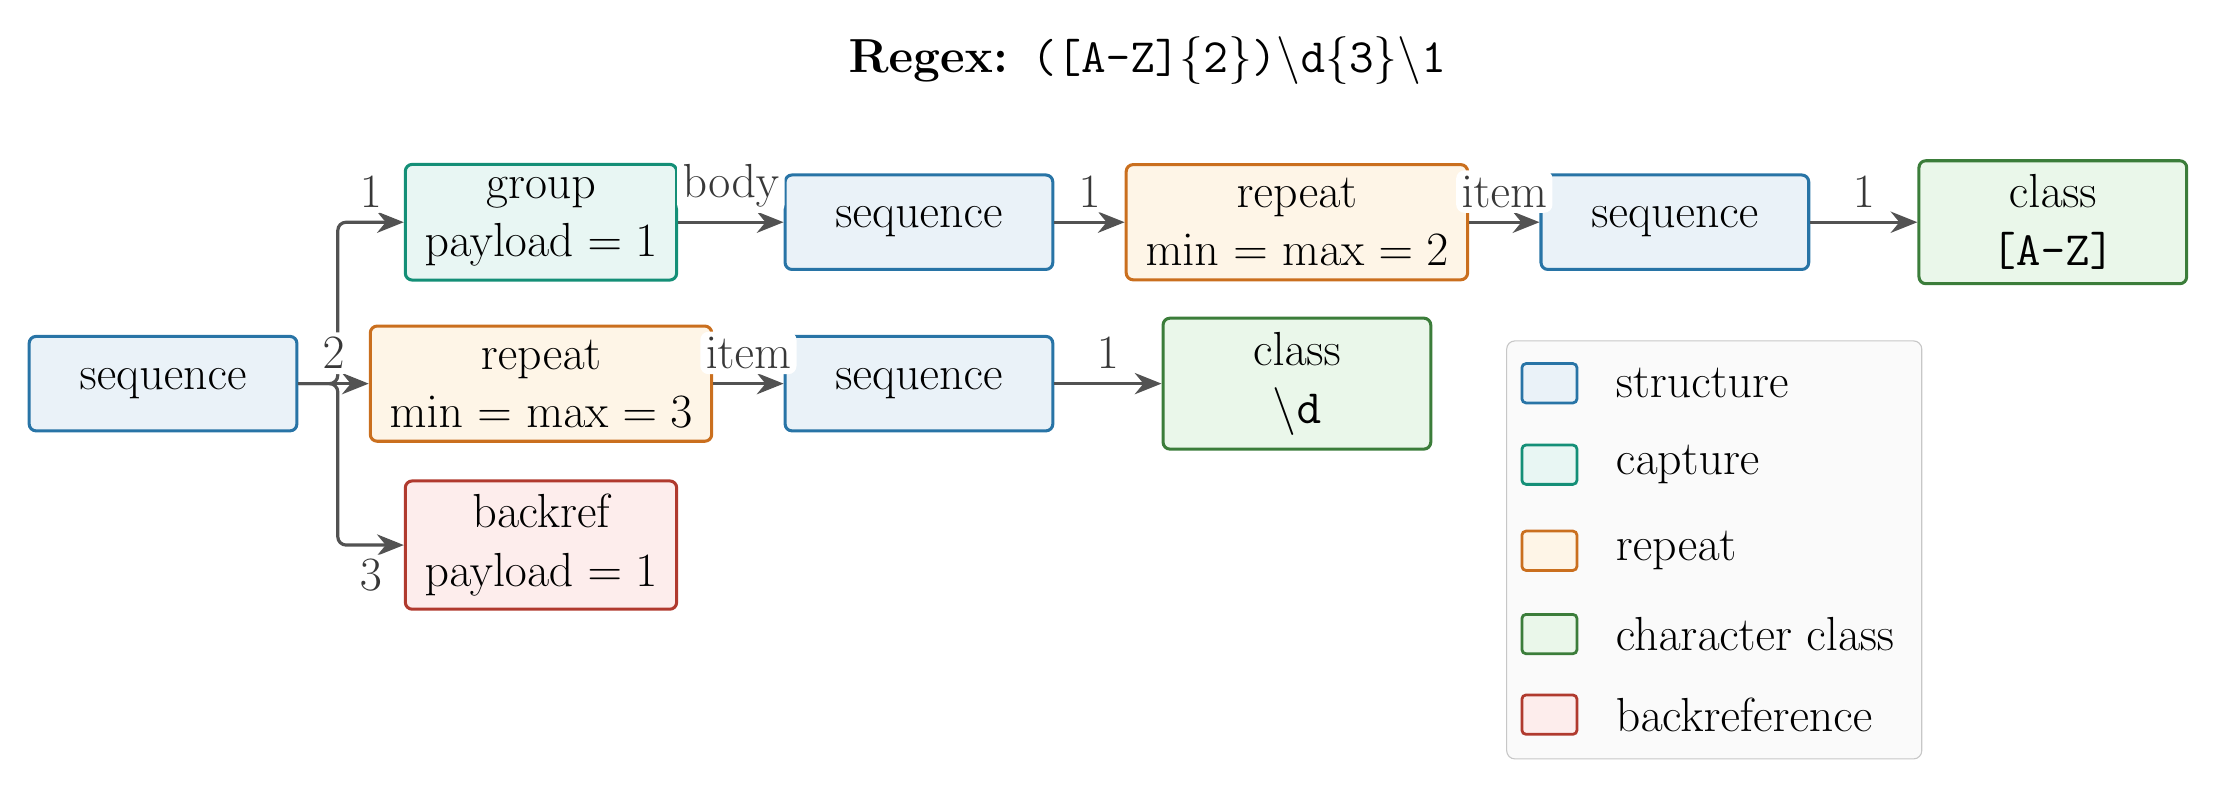
\begin{tikzpicture}[
  font=\fontsize{18}{21}\selectfont,
  >={Stealth[length=3.4mm,width=2.7mm]},
  compact node/.style={
    draw,
    rounded corners=2.5pt,
    line width=1.1pt,
    align=center,
    minimum height=12mm,
    minimum width=34mm,
    inner xsep=7pt,
    inner ysep=5pt
  },
  structural/.style={
    compact node,
    fill=structureFill,
    draw=structureLine
  },
  capture/.style={
    compact node,
    fill=captureFill,
    draw=captureLine
  },
  repeat/.style={
    compact node,
    fill=repeatFill,
    draw=repeatLine
  },
  charclass/.style={
    compact node,
    fill=classFill,
    draw=classLine
  },
  backref/.style={
    compact node,
    fill=backrefFill,
    draw=backrefLine
  },
  edge/.style={
    ->,
    draw=black!68,
    line width=1.15pt,
    rounded corners=3pt
  },
  edge label/.style={
    fill=white,
    text=black!78,
    inner sep=2pt,
    font=\fontsize{18}{21}\selectfont
  },
  legend swatch/.style={
    minimum width=7mm,
    minimum height=5mm,
    rounded corners=1.5pt,
    line width=1pt
  }
]

% Pattern heading
\node[font=\fontsize{18}{21}\selectfont\bfseries] (pattern) at (0,4.1)
  {Regex: \texttt{([A-Z]\{2\})\textbackslash d\{3\}\textbackslash 1}};

% Exact CompactRegexGraphBuilder hierarchy. The hierarchy flows left to right
% so all labels remain at 18 pt on the 5-inch-tall page.
\node[structural] (root) at (-12.5,0) {sequence};

\node[capture] (group) at (-7.7,2.05)
  {group\\payload $=1$};
\node[repeat] (digitRepeat) at (-7.7,0)
  {repeat\\min $=$ max $=3$};
\node[backref] (backrefNode) at (-7.7,-2.05)
  {backref\\payload $=1$};

\node[structural] (groupSequence) at (-2.9,2.05) {sequence};
\node[repeat] (letterRepeat) at (1.9,2.05)
  {repeat\\min $=$ max $=2$};
\node[structural] (letterSequence) at (6.7,2.05) {sequence};
\node[charclass] (letterClass) at (11.5,2.05)
  {class\\\texttt{[A-Z]}};

\node[structural] (digitSequence) at (-2.9,0) {sequence};
\node[charclass] (digitClass) at (1.9,0)
  {class\\\texttt{\textbackslash d}};

% Ordered child and containment edges
\draw[edge] (root.east) -- ++(5mm,0) |- node[edge label, near end, above=1mm] {1} (group.west);
\draw[edge] (root.east) -- node[edge label, above=1mm] {2} (digitRepeat.west);
\draw[edge] (root.east) -- ++(5mm,0) |- node[edge label, near end, below=1mm] {3} (backrefNode.west);

\draw[edge] (group) -- node[edge label, above=1mm] {body} (groupSequence);
\draw[edge] (groupSequence) -- node[edge label, above=1mm] {1} (letterRepeat);
\draw[edge] (letterRepeat) -- node[edge label, above=1mm] {item} (letterSequence);
\draw[edge] (letterSequence) -- node[edge label, above=1mm] {1} (letterClass);

\draw[edge] (digitRepeat) -- node[edge label, above=1mm] {item} (digitSequence);
\draw[edge] (digitSequence) -- node[edge label, above=1mm] {1} (digitClass);

% Compact legend in the otherwise empty backreference branch
\matrix[
  matrix of nodes,
  anchor=north,
  at={(7.2,0.55)},
  draw=black!22,
  rounded corners=3pt,
  fill=black!2,
  inner sep=5pt,
  row sep=2.5mm,
  column sep=3mm,
  nodes={anchor=west, font=\fontsize{18}{21}\selectfont}
] (legend) {
  \node[legend swatch, fill=structureFill, draw=structureLine] {}; & \node {structure}; \\
  \node[legend swatch, fill=captureFill, draw=captureLine] {}; & \node {capture}; \\
  \node[legend swatch, fill=repeatFill, draw=repeatLine] {}; & \node {repeat}; \\
  \node[legend swatch, fill=classFill, draw=classLine] {}; & \node {character class}; \\
  \node[legend swatch, fill=backrefFill, draw=backrefLine] {}; & \node {backreference}; \\
};

\end{tikzpicture}
\end{document}
